%%%%%%%%%%%%%%%%%%%%%%%%%%%%%%%%%%%%%%%%%%%%%%%%%%%%%%%%%%%%%%%%%%%%%
%
% cours Intro à l'optimisation pour le machine learning
%
%%%%%%%%%%%%%%%%%%%%%%%%%%%%%%%%%%%%%%%%%%%%%%%%%%%%%%%%%%%%%%%%%%%%%

\documentclass[12pt]{beamer}
\usepackage[utf8]{inputenc}
\usepackage{amsmath}
\usepackage{amsfonts}
\usepackage{amssymb}
\usepackage{graphicx}
\graphicspath{{figures/}}
%\usepackage{beamerthemesplit}
%\usepackage{beamerthemeshadow} 
\usepackage{color}
\usepackage{hyperref}
\usepackage{xspace}
\usepackage{xifthen}
\usepackage{multicol}
\usepackage{mathtools}
\usepackage{algorithm,algorithmic}
\usepackage{dsfont}
%
% these 2 next needed for mathbb greek letters
\usepackage{breqn} 
\usepackage[bbgreekl]{mathbbol}
%
\usepackage{bbm} % this one is needed for the indicator
%
\usepackage{tikz}
\usetikzlibrary{calc,shapes,arrows,positioning}
%
% handwritten font
\newcommand*{\hwfont}{\fontfamily{qzc}\selectfont}
\DeclareTextFontCommand{\texthw}{\hwfont}

% custom commands in sty file, for easier writting and change of notations
\usepackage{my_notations}

\usetheme{Madrid}
\usecolortheme{beaver}

%%%%%%%%%%%%%%%%%%%%%%%%%%%%%%%%%%%%%%%%%%%%%%%%%%%%%%%%%%%%%%%%%%%%%
\begin{document}
\title
[~Optimisation pour le machine learning
%\hspace{0.5cm}
%\insertframenumber/\inserttotalframenumber
]
{Introduction à l'optimisation pour le machine learning}
\author
[Le Riche et al.]
{\large Rodolphe Le Riche$^1$, Dédji Brian Whannou$^2$, Espéran Padonou$^3$} 
\institute[CNRS/fondat. Vallet]{
$^1$ CNRS LIMOS at Mines Saint-Etienne, France \\
$^2$ KPMG France \\
$^3$ Fondation Vallet
} 
\date[Juillet 2021]{Juillet 2021 \\
Ecole d'Eté en Intelligence Artificielle \\
fondation Vallet\\
Cotonou, Bénin} 
\begin{frame}
\titlepage
\end{frame}

\section{Introduction}
\subsection{Objectifs, remerciements}

%%%%%%%%%%%%%%%%%%%%%%%%%%%%%%%%%%%%%%%%%%%%%%%%%%%%%%%%%%%%%%%%%%
\begin{frame}%[allowframebreaks]
\frametitle{Plan du cours} 
%\begin{multicols}{2}
\begin{center} \textbf{Introduction à l'optimisation pour le machine learning} \end{center}
\tableofcontents[currentsection]
%\end{multicols}
\end{frame}

%%%%%%%%%%%%%%%%%%%%%%%%%%%%%%%%%%%%%%%%%%%%%%%%%%%%%%%%%%%%%%%%%
\begin{frame}
\frametitle{Objectifs du cours}
\begin{itemize}
\item Donner des bases pour l'optimisation numérique
\item en faisant le lien avec le machine learning
\item pour un public de bac+1
\item avec quelques exemples de programmes en R/python codés à partir de 0.
\item Limites: les algorithmes ne seront pas exactement ceux utilisés en pratique pour le deep learning, mais les principaux concepts y seront.
\end{itemize}
\end{frame}

%%%%%%%%%%%%%%%%%%%%%%%%%%%%%%%%%%%%%%%%%%%%%%%%%%%%%%%%%%%%%%%%%
\begin{frame}
\frametitle{Bibliographie du cours}
{\small
Ce cours doit beaucoup à
\begin{itemize}
\item \cite{minoux2008programmation} : un classique sur l'optimisation, écrit avant l'avènement du machine learning mais une vraie base (niveau bac+3)
\item \cite{ravikumar17} : présentation détaillée des algorithmes d'optimisation utiles en machine learning (niveau bac+3)
\item \cite{bishop2006pattern} : un excellent livre d'introduction au machine learning avec quelques commentaires sur l'optimisation (niveau bac+3)
\item \cite{schmidt2007fast} : techniques pour la régularisation L1 (article de recherche)
\item \cite{sun2019optimization} : panorama des méthodes d'optimisation pour les réseaux de neurones, rétro-propagation de gradient (article de recherche)
\end{itemize}
Nous en simplifierons le contenu et emprunterons des illustrations.
} % end small font
\end{frame}

\subsection{Formulation d'un problème d'optimisation}

%%%%%%%%%%%%%%%%%%%%%%%%%%%%%%%%%%%%%%%%%%%%%%%%%%%%%%%%%%%%%%%%%
\begin{frame}
\frametitle{Optimisation = formalisation de la décision}
L'optimisation est une\footnote{non unique, contestable par rapport à l'humain et la vie} formalisation mathématique de la décision
\vskip\baselineskip
\mbox{
\begin{minipage}[c]{0.3\textwidth}

\includegraphics[width=\textwidth]{decision-clipart.jpg}
\end{minipage}
\begin{minipage}[c]{0.7\textwidth}
\begin{equation*}
\min_{x \in \mathcal S} f(x)
\end{equation*}
\begin{itemize}
\item $x$ vecteur des paramètres de la décision~: dimensions, somme investie, réglage d'une machine/code, \ldots
\item $f(x)$~: coût de la décision $x$
\item $\mathcal S$~: ensemble des valeurs possibles de $x$, espace de recherche
\end{itemize}
\end{minipage}
} % end mbox
\end{frame}

%%%%%%%%%%%%%%%%%%%%%%%%%%%%%%%%%%%%%%%%%%%%%%%%%%%%%%%%%%%%%%%%%
\begin{frame}
\frametitle{Optimization example: design}
\begin{center}
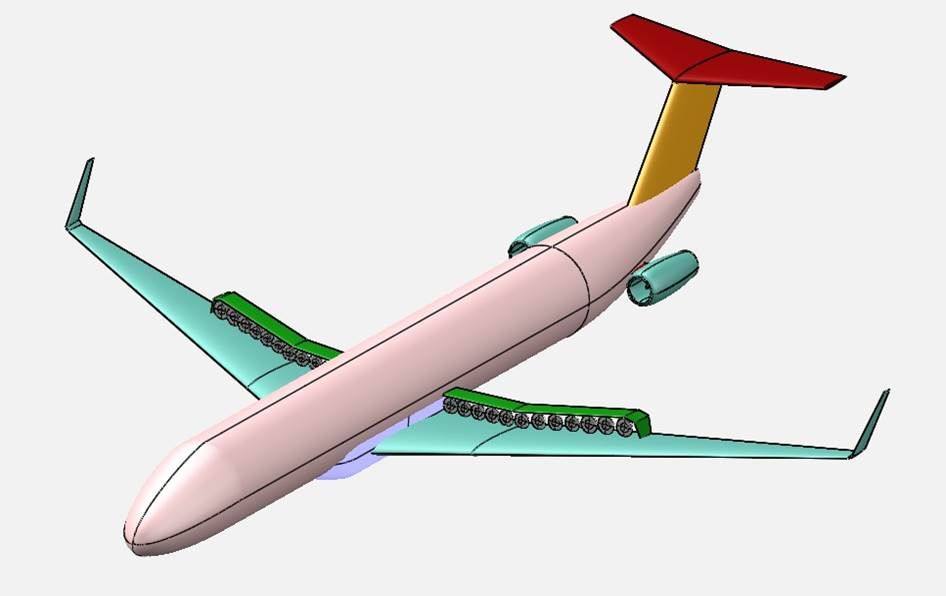
\includegraphics[width=0.5\textwidth]{aircraft_distributed_prop.png}\\
\vspace{-1cm}
{\hfill\tiny (from \cite{sgueglia2018exploration})}
\end{center}
\vskip\baselineskip
$x$ = aircraft parameters (here distributed electrical propulsion)\\
$f()$ = $-1\times$ performance metric (agregation of $-1\times$ range, cost, take-off length, \ldots) \\
At the minimum, the design is ``optimal''.
\end{frame}

%%%%%%%%%%%%%%%%%%%%%%%%%%%%%%%%%%%%%%%%%%%%%%%%%%%%%%%%%%%%%%%%%
\begin{frame}
\frametitle{Optimization example: model identification}
\begin{center}
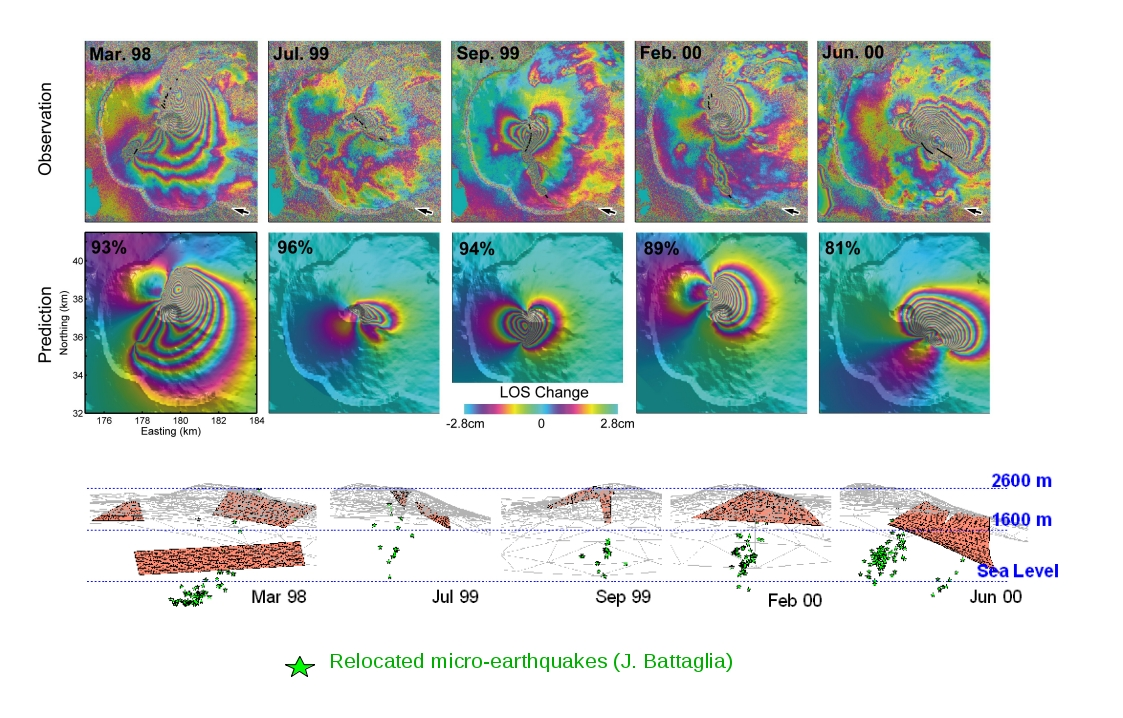
\includegraphics[width=0.7\textwidth]{piton_fournaise.jpg}\\
\vspace{-1cm}
{\hfill\tiny (from \cite{fukushima2010evolution})}
\end{center}
$x$ = dike position, geometry, internal pressure\\
$f()$ = distance between measures (from RADARSAT-1 satellite) and model (boundary elements, non trivial computation)\\
At the minimum, the model best matches measurements and should correspond to the underground phenomenon.
\end{frame}


\subsection{Examples of optimization usages}

%%%%%%%%%%%%%%%%%%%%%%%%%%%%%%%%%%%%%%%%%%%%%%%%%%%%%%%%%%%%%%%%%
\begin{frame}
\frametitle{Optimization example: neural net classification}
\vspace{-0.3cm}
Predict if a person stays at home or goes out based on longitude, latitude and temperature = a 2 classes classification problem.
\begin{center}
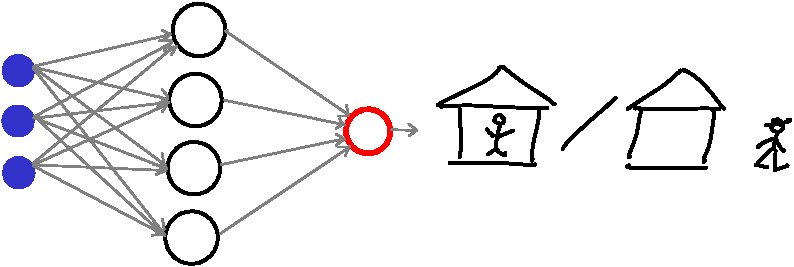
\includegraphics[width=0.6\textwidth]{neuralnet3-4-1-classif-crop.pdf}\\
\vspace{-0.5cm}
\end{center}
$x$ = neural network (NN) weights and biases\\
$f()$ = an error of the NN predictions (a cross-entropy error):
\begin{itemize}
\item $e$ entries: $e_1$ longitude, $e_2$ latitude, $e_3$ temperature
\item $t=1$ if person stays, $t=0$ otherwise
\item Observed data set: $(e^i,t^i),~ i=1,\ldots,N$
\item $y(e;x)$: output of the NN, the probability that $t(e)=1$ 
\item $f(x) = - \sum_{i=1}^N \{ t^i \log(y(e^i;x)) + (1-t^i) \log(1 - y(e^i;x))\}$
\end{itemize}
\end{frame}

%%%%%%%%%%%%%%%%%%%%%%%%%%%%%%%%%%%%%%%%%%%%%%%%%%%%%%%%%%%%%%%%%
\begin{frame}
\frametitle{\small (a word on the classification cross-entropy error)}
\begin{itemize}
\item View the relationship between the entry $e$ and the class $t$ as probabilistic (generalizes deterministic functions): $t(e)$ is a Bernoulli variable with a given probability that $t(e)=1$
\item The NN models this probability: $y(e;x)$ is the probability that $t(e)=1$, $1-y(e;x)$ is the proba that $t(e)=0$, $0\le y(e;x) \le 1$.
\item The probability of $t$ knowing $e$ can be written $y(e;x)^{t}+(1-y(e;x))^{1-t}$
\item The likelihood of the $N$ i.i.d observations is $\prod_{i=1}^N \left[y(e^i;x)^{t^i}+(1-y(e^i;x))^{1-t^i}\right]$, to be maximized
\item The likelihood is turned into an error, to be minimized, by taking $-\log(\text{likelihood})$, 
\begin{equation*}
f(x) = - \sum_{i=1}^N \{ t^i \log(y(e^i;x)) + (1-t^i) \log(1 - y(e^i;x))\}
\end{equation*}
\end{itemize}
\end{frame}

%%%%%%%%%%%%%%%%%%%%%%%%%%%%%%%%%%%%%%%%%%%%%%%%%%%%%%%%%%%%%%%%%
\begin{frame}
\frametitle{Optimization example: neural net regression}
\vspace{-0.3cm}
learn a function from a discrete limited set of observations
%\begin{center}
%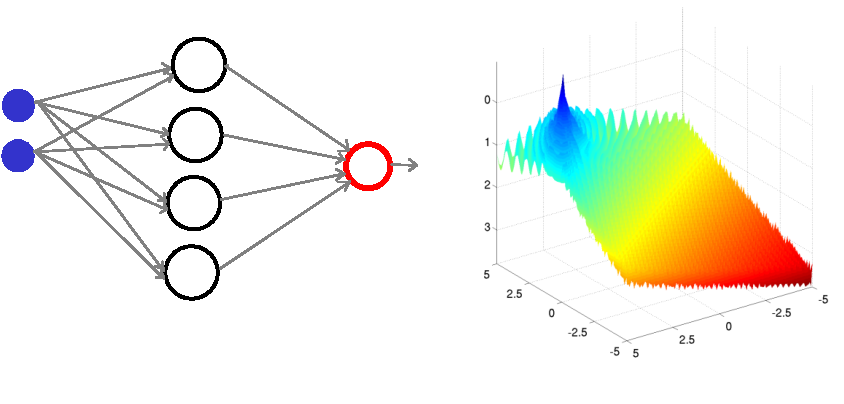
\includegraphics[width=0.6\textwidth]{neuralnet3-4-1-regress-crop.pdf}\\
%\vspace{-0.5cm}
%\end{center}
\begin{center}
\begin{minipage}{0.6\textwidth}
\begin{tikzpicture}
\node[anchor=south west,inner sep=0, outer sep=0] (contour) at (0,0) {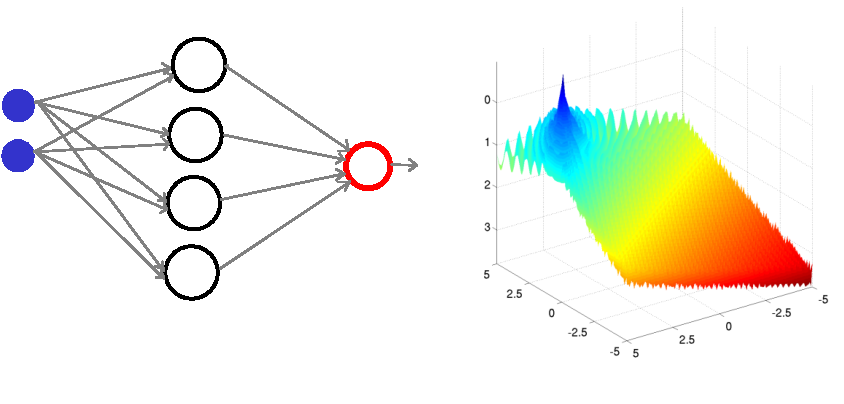
\includegraphics[width=\textwidth]{neuralnet3-4-1-regress-crop.pdf}};
\begin{scope}[x={(contour.south east)},y={(contour.north west)}]
%\draw[help lines,xstep=0.1,ystep=0.1] (0,0) grid (1,1);
\node[] (e1) at (0.6,0.2) {\small $e_1$};
\node[] (e2) at (0.9,0.15) {\small $e_2$};
\node[] (t) at (0.6,0.85) {\small $t(e)$};
\node[] (e1NN) at (-0.05,0.75) {\small $e_1$};
\node[] (e2NN) at (-0.05,0.60) {\small $e_2$};
\node[] (yy) at (0.48,0.69) {\small $y(e \mathchar\numexpr"6000+`;\relax x)$};
\draw[black,fill=black] (0.6,0.63) circle (.15ex);
\draw[black,fill=black] (0.9,0.35) circle (.15ex);
\draw[black,fill=black] (0.665,0.78) circle (.15ex);
\draw[black,fill=black] (0.78,0.7) circle (.15ex);
\draw[black,fill=black] (0.7,0.5) circle (.15ex);
\draw[black,fill=black] (0.85,0.55) circle (.15ex);
\draw[black,fill=black] (0.75,0.35) circle (.15ex);
\end{scope}
\end{tikzpicture}
\end{minipage}
\end{center}
\vspace{-0.5cm}
$x$ = neural network (NN) weights and biases\\
$f()$ = an error of the NN predictions (sum-of-squares error):
\begin{itemize}
\item $e$ entries, $t(e)$ target function to learn
\item observed data set, ``\tikz\draw[black,fill=black] (0,0) circle (.15ex);'' : $(e^i,t^i),~ i=1,\ldots,N$
\item $y(e;x)$: output of the NN, the expected value of $t(e)$ 
\item $f(x) = 1/2 \sum_{i=1}^N (t^i - y(e^i;x))^2 $
\end{itemize}
\end{frame}

%%%%%%%%%%%%%%%%%%%%%%%%%%%%%%%%%%%%%%%%%%%%%%%%%%%%%%%%%%%%%%%%%
\begin{frame}
\frametitle{Optimization example: image denoising}
\vspace{-0.5cm}
\begin{equation*}
\begin{split}
\min_x f(x) \quad,\quad & f(x) = \frac{1}{2}\sum_{i=1}^{N_{\text{pixels}}} (y_i - x_i)^2 + 
\lambda \sum_{i=1}^{N_{\text{pixels}}} \sum_{j \text{ near } i} \lvert x_i - x_j \rvert \\
& \lambda \ge 0 \quad\text{regularization constant}
\end{split}
\end{equation*}
\begin{center}
\begin{minipage}[t]{0.2\textwidth}

\includegraphics[width=\textwidth]{c_clean.png} \\
{\small target image}
\end{minipage}
\hfill
\begin{minipage}[t]{0.2\textwidth}
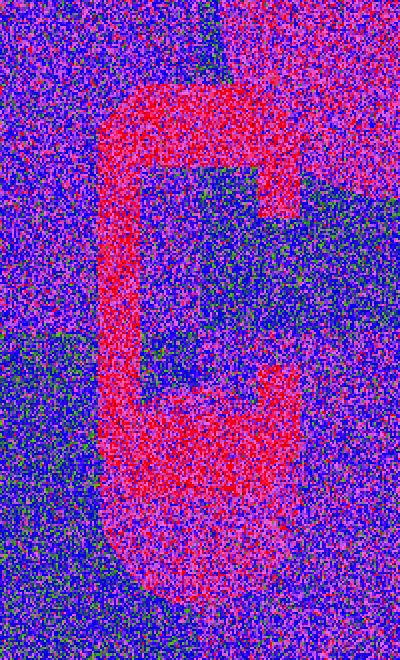
\includegraphics[width=\textwidth]{c_noisy.png} \\
{\small \mbox{noisy (observed)} $= y_i$'s}
\end{minipage}
\hfill
\begin{minipage}[t]{0.2\textwidth}

\includegraphics[width=\textwidth]{c_denoised.png} \\
{\small \mbox{denoised (optimized)} $=x^\star$}
\end{minipage}
\mbox{\quad}
\end{center}
{\scriptsize (from \cite{ravikumar17}) \hfill}
\end{frame}


\subsection{Optimization basics}

%%%%%%%%%%%%%%%%%%%%%%%%%%%%%%%%%%%%%%%%%%%%%%%%%%%%%%%%%%%%%%%%%%
\begin{frame}%[allowframebreaks]
\frametitle{Optimization basics} 
%\begin{multicols}{2}
\tableofcontents[currentsection]
%\end{multicols}
\end{frame}

%%%%%%%%%%%%%%%%%%%%%%%%%%%%%%%%%%%%%%%%%%%%%%%%%%%%%%%%%%%%%%%%%%
\begin{frame}
\frametitle{Local versus global optimum} 
\begin{equation*}
\min_{x \in \mathcal S \subset \Rset[d]} f(x)
\end{equation*}
\vspace{-0.4cm}
\begin{center}
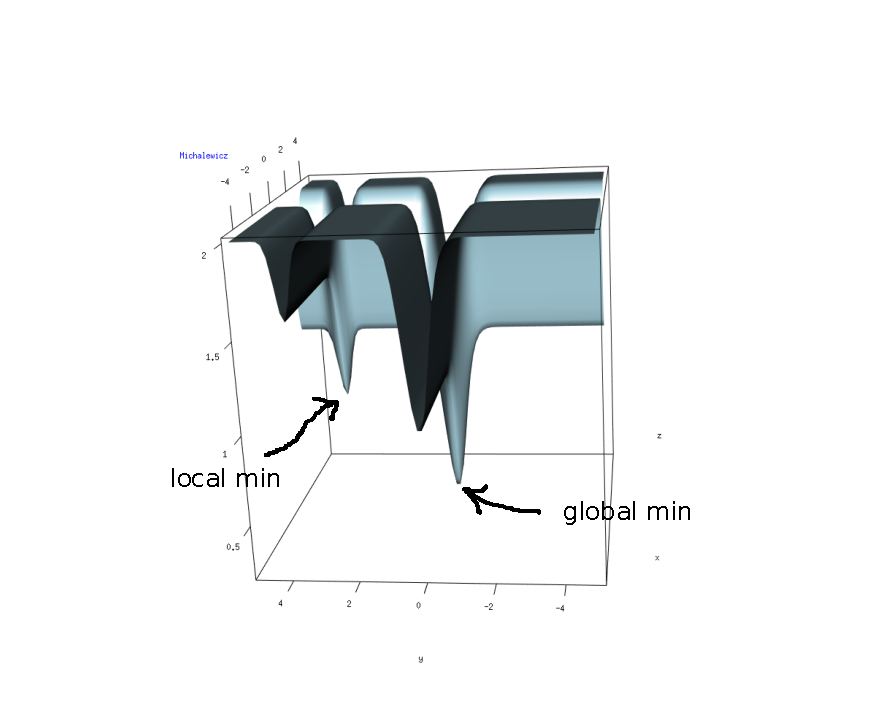
\includegraphics[width=0.7\textwidth]{michalewicz_function_annotated-crop.pdf} \\
\end{center}
\vspace{-1.cm}
R code to generate the plot given in the project folder
\end{frame}

%%%%%%%%%%%%%%%%%%%%%%%%%%%%%%%%%%%%%%%%%%%%%%%%%%%%%%%%%%%%%%%%%%
\begin{frame}
\frametitle{Gradient of a function} 
Gradient of a function = direction of steepest ascent = vector of partial derivatives
\begin{equation*}
\nabla f(x) = \begin{pmatrix} \frac{\partial f}{\partial x_1}(x) \\ \ldots \\ \frac{\partial f}{\partial x_d}(x) \end{pmatrix}
\end{equation*}
\begin{center}
\begin{minipage}[t]{0.7\textwidth}
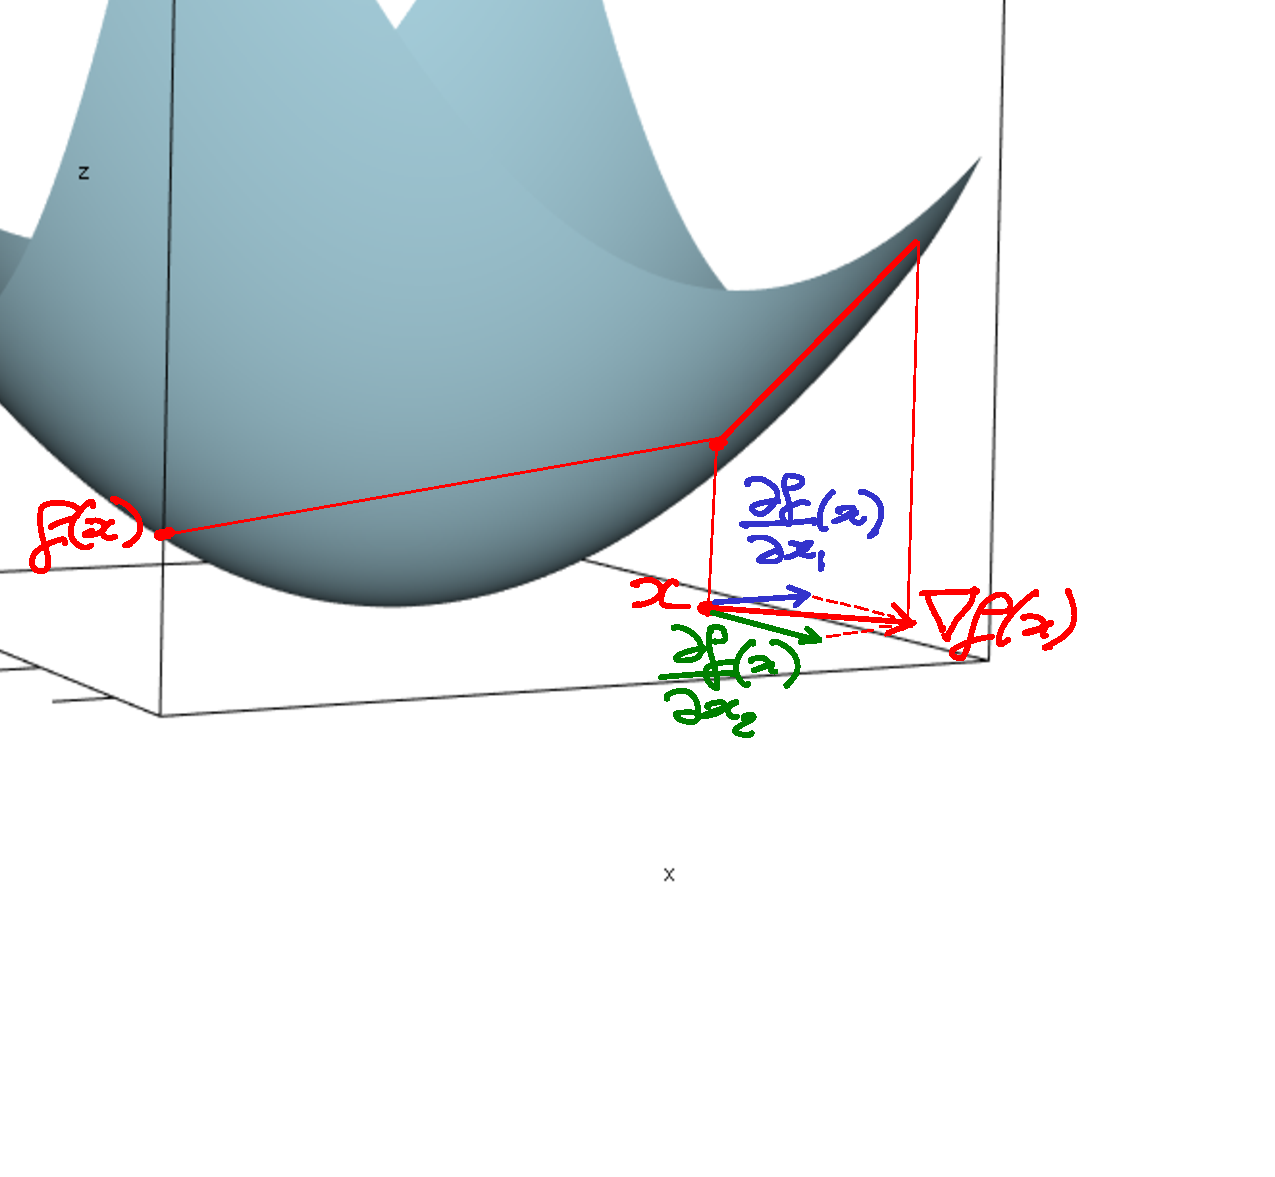
\includegraphics[width=\textwidth]{gradient-crop.pdf} \\
\end{minipage}
\end{center}
\end{frame}

%%%%%%%%%%%%%%%%%%%%%%%%%%%%%%%%%%%%%%%%%%%%%%%%%%%%%%%%%%%%%%%%%%
\begin{frame}
\frametitle{Numerical approximation of the gradient} 
\mbox{
\begin{minipage}[b]{0.6\textwidth}
By forward finite differences 
\begin{equation*}
\frac{\partial f}{\partial x_i}f(x) \approx \frac{f(x+h e^i)-f(x)}{h}
\end{equation*}
{Proof: \scriptsize
 by Taylor,\\
$f(x+he^i) = f(x) + h {e^i}^\top \nabla f(x) + h^2/2 {e^i}^\top \nabla^2 f(x+\rho h e^i) e^i~,~\rho\in ]0,1[$ \\
$\nabla f(x) = \frac{f(x+he^i)-f(x)}{h} - h/2 {e^i}^\top \nabla^2 f(x+\rho h e^i) e^i $ \\
and make $h$ very small $\square$
}
\end{minipage}
\begin{minipage}[b]{0.4\textwidth}
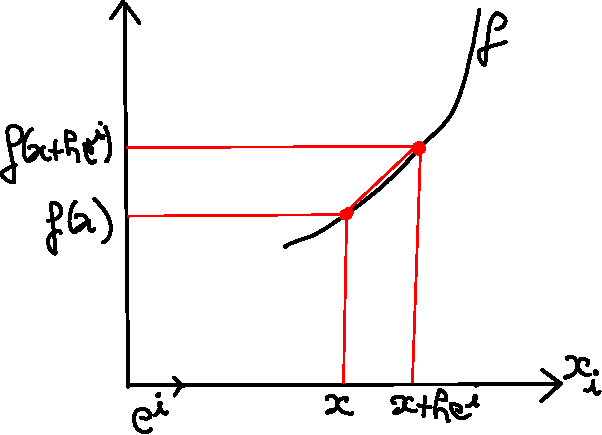
\includegraphics[width=\textwidth]{finitediff-crop.pdf}
\end{minipage}
} % mbox
\vskip\baselineskip
Other (better but more difficult to implement) schemes: central differences, automatic differentiation (e.g., in TensorFlow or PyTorch), (semi-)analytic differentiation (e.g., backpropagation in NN).
\end{frame}

%%%%%%%%%%%%%%%%%%%%%%%%%%%%%%%%%%%%%%%%%%%%%%%%%%%%%%%%%%%%%%%%%%
\begin{frame}
\frametitle{Descent direction} 
\mbox{
\begin{minipage}[b]{0.5\textwidth}
A search direction $d$ which makes an acute angle with $-\nabla f(x)$ is a descent direction, i.e., for a small enough step $f$ is guaranteed to decrease!
\end{minipage}
\hfill
\begin{minipage}[t]{0.4\textwidth}
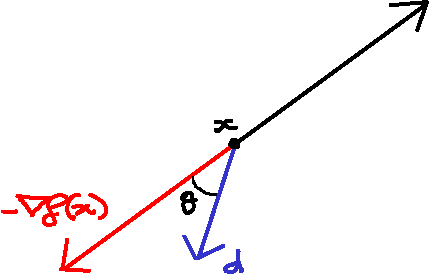
\includegraphics[width=\textwidth]{descent_direction-crop.pdf}
\end{minipage}
}
\\\vspace{0.8cm}
{\normalsize
Proof: by Taylor, $\forall \alpha \le 0,~\exists \epsilon \in [0,1]$ such that
$f(x+\alpha d) = f(x) + \alpha d^\top \nabla f(x) + \frac{\alpha^2}{2} d^\top \nabla^2f(x + \alpha \epsilon d) d$\\
$\lim_{\alpha \rightarrow 0^+} \frac{f(x+\alpha d) - f(x)}{\alpha} = d^\top \nabla f(x) = - 1\times \lVert \nabla f(x)\rVert \cos(d,-\nabla f(x))$ \\
is negative if the cosine is positive $\square$
} %end small
\end{frame}

%%%%%%%%%%%%%%%%%%%%%%%%%%%%%%%%%%%%%%%%%%%%%%%%%%%%%%%%%%%%%%%%%%
\begin{frame}
\frametitle{Necessary optimality condition (1)} 
A necessary condition for a differentiable function to have a minimum at $x^\star$ is that it is flat at this point, i.e., its gradient is null
\begin{equation*}
x^\star \in \arg \min_{x \in \mathcal S} f(x) \Rightarrow \nabla f(x^\star) = 0
\end{equation*}
\vskip\baselineskip
\begin{center}
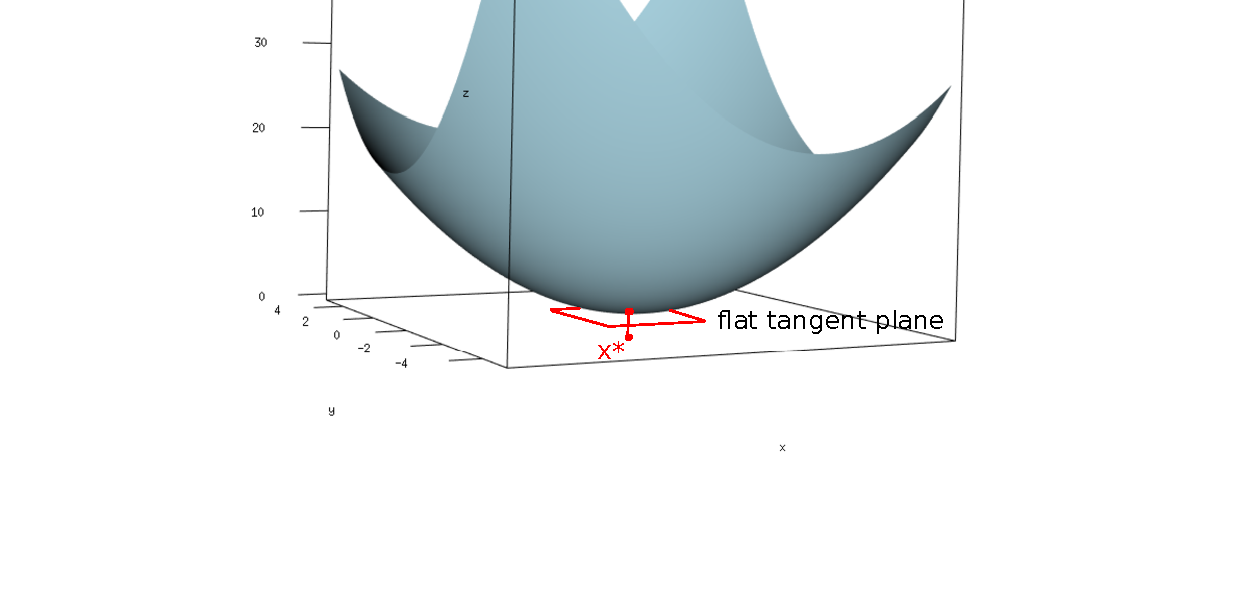
\includegraphics[width=1.2\textwidth]{minimum-crop.pdf} \\
\end{center}
\end{frame}

%%%%%%%%%%%%%%%%%%%%%%%%%%%%%%%%%%%%%%%%%%%%%%%%%%%%%%%%%%%%%%%%%%
\begin{frame}
\frametitle{Necessary optimality condition (2)} 
\begin{center}
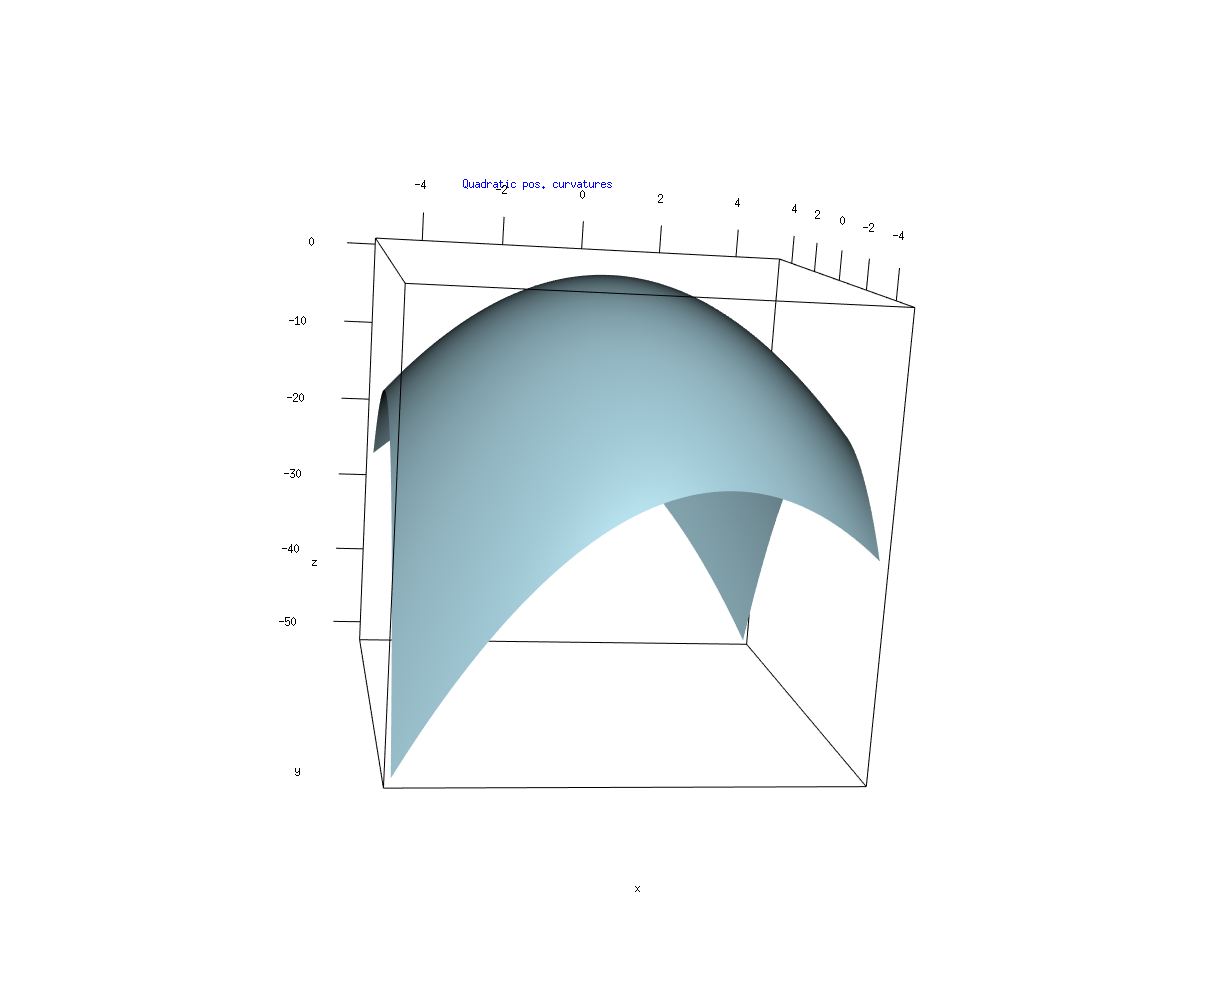
\includegraphics[width=0.7\textwidth]{quad_neg_curv.png} \\
necessary is not sufficient (works with a max) 
\vspace{2cm}
\end{center}
\end{frame}

%%%%%%%%%%%%%%%%%%%%%%%%%%%%%%%%%%%%%%%%%%%%%%%%%%%%%%%%%%%%%%%%%%
\begin{frame}
\frametitle{Necessary optimality condition (3)} 
\begin{center}
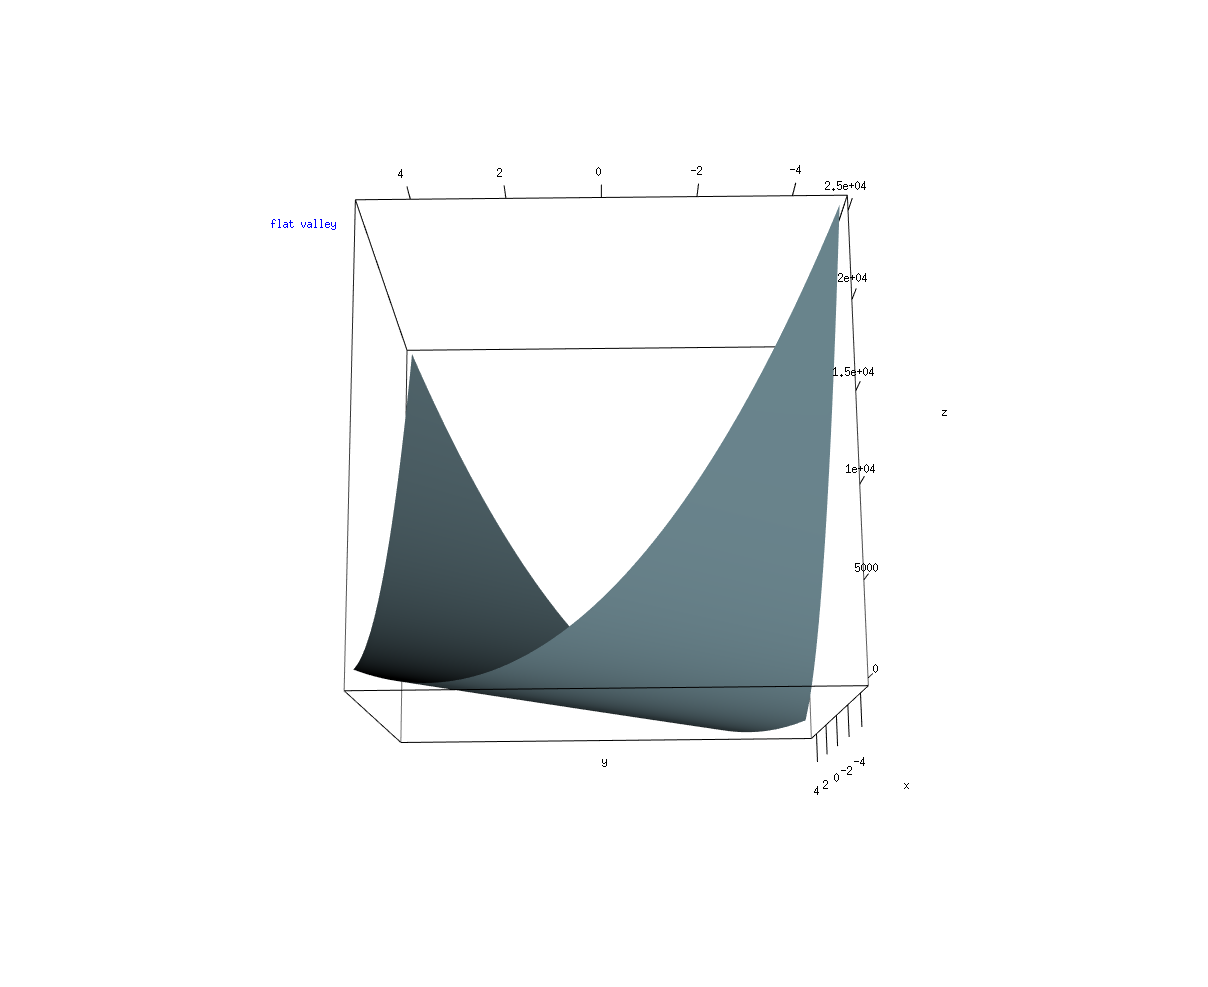
\includegraphics[width=0.7\textwidth]{flat_valley.png} \\
$\nabla f(x^\star) = 0$ does not make $x^\star$ unique (flat valley)
\end{center}
\end{frame}

%%%%%%%%%%%%%%%%%%%%%%%%%%%%%%%%%%%%%%%%%%%%%%%%%%%%%%%%%%%%%%%%%%
\begin{frame}
\frametitle{Necessary optimality condition (4)} 
\begin{center}
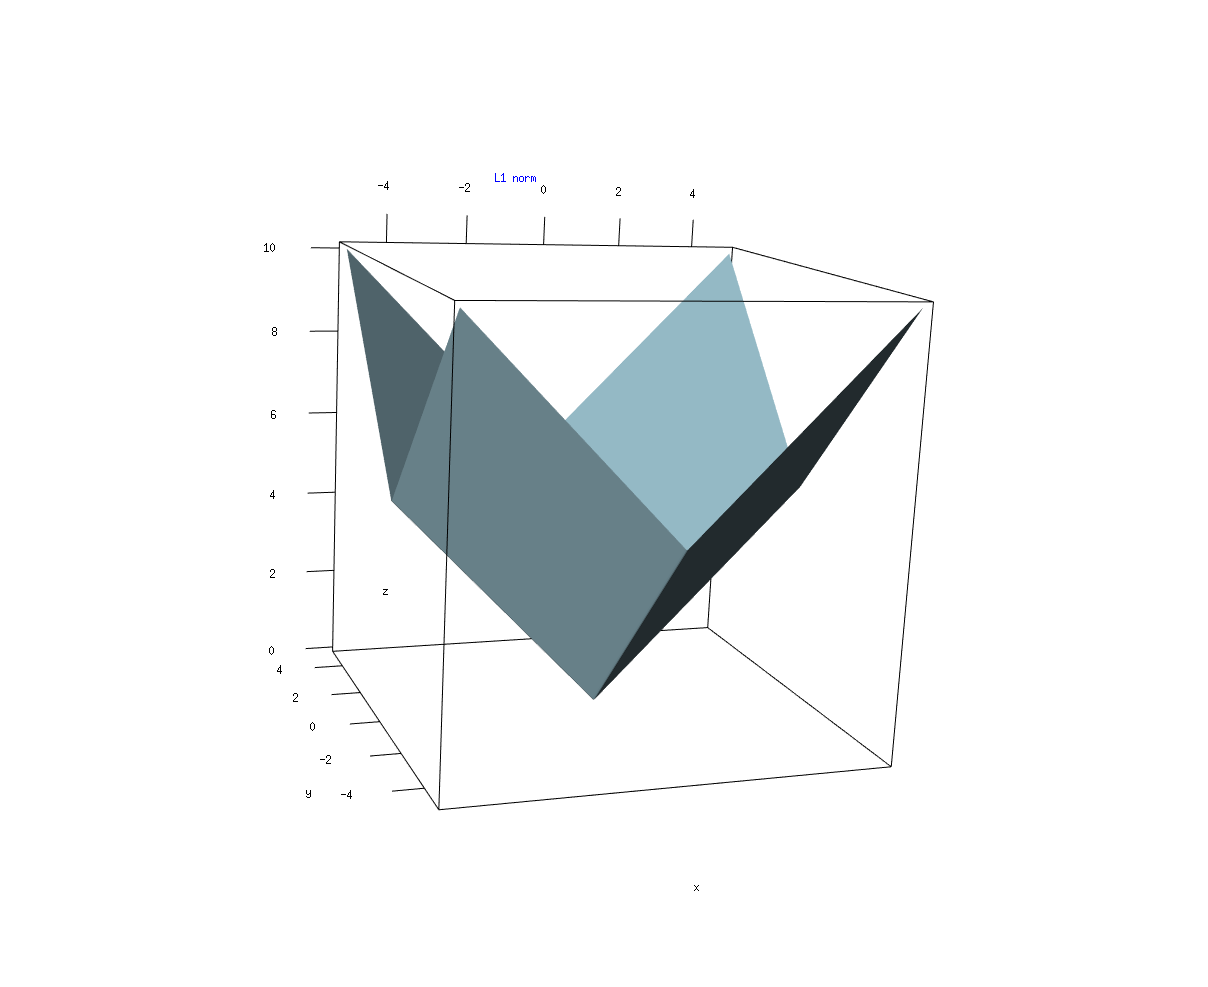
\includegraphics[width=0.7\textwidth]{L1norm.png} \\
$\nabla f()$ not defined everywhere, example with L1 norm $= \sum_i^d \lvert x_i \rvert$
\end{center}
\end{frame}

\section{Steepest descent}

%%%%%%%%%%%%%%%%%%%%%%%%%%%%%%%%%%%%%%%%%%%%%%%%%%%%%%%%%%%%%%%%%%
\begin{frame}%[allowframebreaks]
\frametitle{Plan du cours} 
%\begin{multicols}{2}
\begin{center} \textbf{An introduction to optimization for machine learning} \end{center}
\tableofcontents[currentsection]
%\end{multicols}
\end{frame}

\subsection{Algorithm}

%%%%%%%%%%%%%%%%%%%%%%%%%%%%%%%%%%%%%%%%%%%%%%%%%%%%%%%%%%%%%%%%%%
\begin{frame}
\frametitle{Steepest descent algorithm} 
\textcolor{red}{(work in progress)}
present algo\\
\end{frame}

%%%%%%%%%%%%%%%%%%%%%%%%%%%%%%%%%%%%%%%%%%%%%%%%%%%%%%%%%%%%%%%%%%
\begin{frame}
\frametitle{Comments on steepest descent} 
\textcolor{red}{(work in progress)}
show that (with perfect line search) consecutive search directions are perpendicular: tendency to oscillate, sensitive to bad conditionning\\
other flaws: no convergence on nondifferentiable functions, gets trapped in local minima
\end{frame}

\subsection{Application neural network}

\section{Improved gradient searches}
%%%%%%%%%%%%%%%%%%%%%%%%%%%%%%%%%%%%%%%%%%%%%%%%%%%%%%%%%%%%%%%%%%
\begin{frame}%[allowframebreaks]
\frametitle{Plan du cours} 
%\begin{multicols}{2}
\begin{center} \textbf{An introduction to optimization for machine learning} \end{center}
\tableofcontents[currentsection]
%\end{multicols}
\end{frame}

\section{Prise en compte des contraintes d'optimisation}
%%%%%%%%%%%%%%%%%%%%%%%%%%%%%%%%%%%%%%%%%%%%%%%%%%%%%%%%%%%%%%%%%%
\begin{frame}%[allowframebreaks]
\frametitle{Plan du cours} 
%\begin{multicols}{2}
\begin{center} \textbf{Introduction à l'optimisation pour le machine learning} \end{center}
\tableofcontents[currentsection]
%\end{multicols}
\end{frame}

\section{Conclusions}

%%%%%%%%%%%%%%%%%%%%%%%%%%%%%%%%%%%%%%%%%%%%%%%%%%%%%%%%%%%%%%%%%
\begin{frame}
\frametitle{Conclusions}
\begin{itemize}
\item L'optimisation numérique est une technique fondamentale associée à la décision optimale et à la modélisation statistique (machine learning).
\item Avec l'enthousiasme autour du machine learning, de nombreux algorithmes ont été conçus que nous n'avons pas couverts ici: l'optimisation bayésienne (Bayesian optimization) pour le réglage des hyper-paramètres (paramètres de régularisation, nombre de couches du réseau de neurone, type de neurones, paramètres de l'algorithme d'optimisation des poids).
\end{itemize}
\end{frame}

\section{Bibliography}

%=======================================================================================
\begin{frame}[allowframebreaks]
\frametitle{References}
\scriptsize
%\vspace{-1.cm}
%\setbeamertemplate{bibliography item}{[\theenumiv]} % to have numbers in biblio with beamer
%   \bibliographystyle{plain}
   \bibliographystyle{apalike}
   \bibliography{biblio}
\end{frame}

\end{document}
